\chapter{Description of the domain of analyzed conference paper reviews}
The data on which the analysis will be done are all from events and conferences focused on semantic technology (ST). Sentiment analysis is usually applied to product reviews or posts on social media, therefore this work will serve as an exploration of the possibility of creating a  model which, even though focused on one domain, is generalized  across various events of the same umbrella subject.

Eventually, the model can be extended to be less domain-specific, given that the review metrics probably will not differ significantly between different research areas. 

In this chapter I want to give you a brief introduction into the studied domain of conferences with focus on semantic technology INSERT MORE TEXT.

\section{Studied conferences within the field of semantic technology}
\subsection{European Semantic Web Conference ESWC}
The European Semantic Web Conference (ESWC) is an international conference on the topic of ST which first began in 2004.
According to the ESWC website, ``the mission of the ESWC is to bring together researchers and practitioners in all these areas dealing with different aspects of semantics on the Web.''\cite{eswc}.

The topics of ESWC conferences include linked open data, machine learning, natural language processing and information retrieval, ontologies, reasoning, semantic data management, services, processes, and cloud computing, social Web and Web science, in-use and industrial, digital libraries and cultural heritage, and e-government.\cite{eswc_topics}
\subsection{European Knowledge Acquisition Workshop EKAW}
The European Knowledge Acquisition Workshop (EKAW) started in 1987 as a workshop in the field of knowledge-based systems and became a conference in 2000 changing its full title to the International Conference on Knowledge Engineering and Knowledge Management.\cite{ekaw}

As they state on their website about the 2020 EKAW conference ``the 22nd International Conference on Knowledge Engineering and Knowledge Management is concerned with all aspects about eliciting, acquiring, modeling and managing knowledge, and the construction of knowledge-intensive systems and services for the semantic web, knowledge management, e-business, natural language processing, intelligent information integration, and so on''\cite{ekaw_2020}.
\subsection{International Semantic Web Conference ISWC}
The International Semantic Web Conference (ISWC) is a conference with focus on research on semantic web topics including linked data. It is a successor of the Semantic Web Working Symposium (SWWS) and is held annually since 2002.\cite{iswc}


\section{Reviewing process of conference submissions}
The aim of this section is to give an overview of the steps of a reviewing process to give the reader a better understanding on the context in which the reviews analyzed in this work are created.
While the reviewing process of different conferences may vary, there is set of general steps which they all follow to a certain degree. 

Each paper submitted to a conference is reviewed by multiple reviewer (usually three or more). After the reviewers submit their reviews authors may be able to react during a rebuttal phase, by clearing up any misunderstandings, answering questions posed by the reviewers and by defending their position on things a reviewer may have complained about. This is a common reviewing step in bigger conferences such as ISWC or ESWC however that may not be the case for smaller conferences such as EKAW where the authors only get the final reviews and whether the submission was accepted or not. Sometimes the authors get the numerical scores given by the reviewers as well as the written reviews with reviewer's comments, but occasionally only the comments are supplied so as the authors cannot use the numerical scores to argue (for example when the scores given by one reviewer are significantly higher that the scores of other reviewers).

Certain conferences also have an ``offline'' discussion amongst the reviewers, which is not accessible by the authors, which is usually moderated by a track chair.

Based on the reaction of the authors of the papers to the initial reviews the reviewers have the opportunity to adjust their reviews (or they should at least make it clear that they have read the author's response).

The track chair also can write meta reviews, which serve as summaries of the more in-depth reviews by the other reviewers. That is a standard step in conferences where there is also a conference chair above the track chair who makes the final decision about a paper acceptance. In that case the conference chair mostly decides based on the conclusion given in the meta review, it is quite rare for them to decide otherwise.

In terms of anonymity in the reviewing process, there are many different options and situations.  Usually the author is not given the names of reviewers, but reviewers can see the names of the authors. Occasionally conferences follow a double-blind model, where the paper's authorship is anonymized. However that is not always possible, for example resource tracks (tracks aimed at sharing resources including datasets, software frameworks, ontologies, methodologies or metrics) are just about impossible to anonymize due to the fact that the resources the papers refer to need to be publicly available and in use. 

Sometimes conferences however do allow the authors to know the names of the reviewers (albeit the reviewers usually have the option to stay anonymous if the wish).

Certain conferences also keep the reviewers anonymous from one another or from the meta reviewer. The goal here is to give less experienced reviewers a chance to express themselves without worrying about the opinion of senior reviewers and vice versa to keep more experienced reviewers from undermining the opinions given by a less experienced reviewer.
\section{The Structure of conference paper reviews}
\label{sec:rev_structure}
Different conferences structure their reviews differently. Some are in the form of a completely unstructured text, while some clearly separate the comments in the reviews by the criteria. 

For example the structure of the 2018 EKAW conference reviews is that there is a set of criteria which are assigned numeric scores (relevance, overall evaluation and reviewer's confidence) followed by two yes or no scoring (best paper candidate and poster \& demo candidate). It is then followed by a summary of the reviewed paper. The reviewers comments are divided into three parts which are \textit{Reasons to accept}, \textit{Reasons to reject} and \textit{Overall evaluation}. The reviews also sometimes contain confidential remarks for the program committee.

The 2017 ISWC and 2018 ISWC conferences were more detailed with its numerical scoring, assigning these scores to:
\begin{itemize}
\item Reviewer's confidence
\item Appropriateness
\item Clarity and quality of writing
\item Related work
\item Originality/innovativeness
\item Impact of ideas and results
\item Implementation and soundness
\item Evaluation
\item Overall paper evaluation
\end{itemize}

Following these numerical scores, the rest of the ISWC reviews are however in the form of unstructured text, unless the author of the review specifically made the decision to structure their comments either by the judged aspect or by the positivity or negativity of their comments.

The most structured reviews I have had to my disposal to study were from the 2018 ESWC conference. There, numeric score were assigned to:
\begin{itemize}
\item Relevance to ESWC
\item Novelty of the proposed solution
\item Correctness and completeness of the proposed solution
\item Evaluation of the state-of-the-art
\item Demonstration and discussion of the properties of the proposed approach
\item Reproducibility and generality of the experimental study
\item Overall score
\end{itemize}

while the textual part of the review was clearly divided into the same categories.
\section{Previous research on conference paper reviews}
While there is quite a lot of existing research regarding information extraction from research papers, mostly used for paper summarization and extraction of keywords, I could not find much research focused on information extraction or opinion mining from the reviews of such papers. 
In terms of  on possible generic metrics, previous research on this topic was done by \textcite{svatek_strossa} in their paper on the possibility of pictorial representation of review scores. The metrics they propose are these:
\begin{itemize}
    \item Relevance
    \item Novelty
    \item Technical quality
    \item State of the art
    \item Evaluation
    \item Significance
    \item Presentation
\end{itemize}
Their overview of different metrics of nine confereces with focus on semantic technology and knowledge engineering and their mapping onto their set of generic criteria can be found on table \ref{table:conf}.
\begin{landscape}
\begin{table}[p]
\caption[Mapping between generic review metrics and form fields]{Proposed mapping between generic review metrics and form fields of KE conferences\cite{svatek_strossa}}
\label{table:conf}
\small
\centering

\setlength{\defaultaddspace}{.33333\defaultaddspace}
\begin{tabular}
    {   
        L{15mm} | % gencat 
        L{18mm}  % ecai
        L{12mm}  % ekaw   
        L{60mm}  % eswc
        L{20mm}  % fois
        L{18mm}  % ijcai
        L{25mm}  % iswc
        L{16mm}  % kr     
    }
     \toprule
Review metric	&	ECAI (2016)	&	EKAW (2020)	&	ESWC (2018)	&	FOIS (2016)	&	IJCAI (2019) &	ISWC, SEMANTiCS (2018)	&	KR (2014)	\\
     \toprule
Relevance	&	Relevance	&	NA	&	Relevance to ESWC	&	NA	&	Relevance	&	Appropriateness	&	Relevance of the paper to KR	\\
\midrule
Novelty	&	Originality	&	Novelty	&	Novelty of the proposed solution	&	Novelty or innovation	&	Originality	&	Originality / innovativeness	&	Novelty of the contribution	\\
\midrule
Technical quality	&	Technical quality &	Technical soundness and depth &	Correctness and completeness of the proposed solution; Demonstration and discussion of the properties of the proposed approach	&	Scientific or technical quality	&	Technical quality	& Implementation and soundness	&	Technical quality	\\
\midrule
State of the art	&	Scholarship	&	NA	&	Evaluation of the state-of-the-art	&	References	&	Scholarship	&	Related work	&		Discussion of related work	\\
\midrule
Evaluation	&	NA	&	NA	&	Reproducibility and generality of the experimental study	&	NA	&	NA	&	Evaluation	&	NA	\\
\midrule
Significance	&	Significance	&	NA	&	NA	&	NA	&	Significance	&	Impact of ideas and results	&	NA	\\
\midrule
Presentation	&	Presentation quality	&	Clarity and quality of writing	&	NA	&	Presentation &	Clarity and quality of writing	&	Clarity and quality of writing	&		Quality of the presentation	\\
     \bottomrule
\end{tabular}

\end{table}

\end{landscape}
One research I found that was specifically focused on sentiment analysis of reviews of scientific publications was the research done be \textcite{nano_peer}. They used a dataset of eleven reviews, each of which was manually annotated by their respective authors. The aspects of the reviews they focused on were syntax, style and content so each reviewer was asked to which of these aspects a specific comment in their review focused on, whether the comment was positive or negative, whether an action by the author of the paper was required or just suggested, what was the impact for the overall quality of the paper and whether the author addressed the point raised in the comment.\cite{nano_peer} In the eleven reviews there was a total of 421 review comment, most of which (around 44 \%) targeted a paragraph or an even smaller part of the paper, almost 30 \% were about the paper as a whole and 27 \% of comments focused on a section of the paper. 
The first fairly interesting outcome of this study was that the authors of the study also annotated the review comments themselves and they gathered annotations from peer reviewers. The compared the results and the level of disagreement using a variation of the Mean Squared Error metric, calculated as the square root of the mean squared differences between the average responses of the groups for numerical dimensions and as thee the squared
differences from the ratio for each category separately for nominal dimensions. From the results it was clear that ``the model experts and the
peers always agree with each other more than they agree with the
ground truth in the form of the original reviewer'' which according to the authors seems to indicate that ``they misinterpret the review comments in a relatively
small but consistent manner''\cite{nano_peer}.

I also want to include here the result of the annotating phase done by the model experts (the authors), which you can see on figure \ref{img:annotations}. As you can see on the graph most of the review comments are about the content of the paper, with much smaller percentages being comments about the style or the syntax. Also the amount of negative comment far exceeds the number of neutral or positive comments. 

 \ref{img:annotations}.

   \begin{figure}[htbp!]\centering
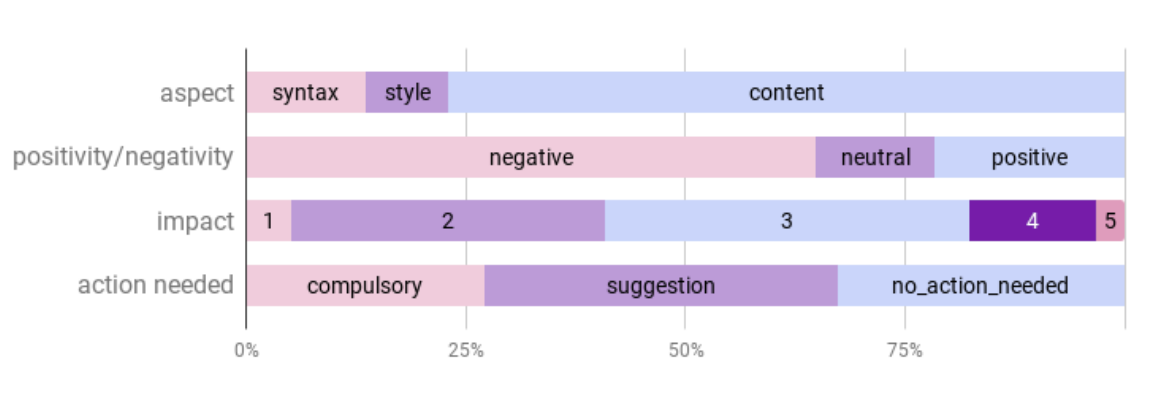
\includegraphics[width=.66\textwidth]{img/nano_annotations}
      \caption[The results of the model expert annotations]{The results of the model expert annotations\cite{nano_peer}}\label{img:annotations}
    \end{figure}
They have applied 18 different lexicon-based sentiment analysis tools to compare the results and found that the best permorming tool was the SOCAL method\cite{socal} with a maximum accuracy of 72.8 \%. Most of the methods performed quite poorly according to the authors, however they discovered that the methods with more complex rules performed the best, even if the size of their sentiment lexicon was not large. It is important to note in the context of this work that the sentiment analysis was done separately from the aspects purely focusing on the polarity of the comment and they did not develop or used any tools to automatically determine the aspect of the comment.

Another research that is focused on the processes of scientific publishing and more importantly peer reviewing of these publications was done by by the same authors as the last paper. This study is focused on creating a unified model for representation of publications and their assessments ``as well as the involved processes, actors, and provenance in general''\cite{nanopublications} in the format of linked data. Their vision is that to give more context to reviews, by linking them to other data, such as information about the reviewer and about the author of a paper, as well as provide a way to link specific parts of a review to the part of the paper they comment on.

In their study they performed a user study based on a set of 7 competency questions to determine the practicality of the ontology they propose. The respondents were ask to judge the importance of each of these questions on a scale form 1 to 5 (1 meaning \textit{not important at all} and 5 \textit{very important}). One of these questions,  was ``What is the distribution of the review comments with respect to whether
they address the content or the presentation (syntax and style) of the article?'' which was given the average importance score of 3.64, which was the second highest importance score in their set of question. This tells me that the focus of my paper might indeed be valuable for the community, as it focuses on an even more fine-grained aspect-based sentiment analysis of the reviews.
